\chapter{System Design}
In this chapter we will discuss the design and architecture of the web-applications system and how the aforementioned technologies are integrated throughout the web-application. Typically in the case of a web-application such as the one defined within this paper, three-tier architecture would be employed as a means to operate the system. However, because Firebase is a backend-as-a-service, technically that would making the architecture of this project 2-tier. However, the two-tier architecture of a Firebase web-application such as this uses pseudo servers, by using imports of angularfire modules, giving the same core functionality as an application with 3-tier architecture. 

\section{Overview}
To describe this application in terms of a 3-tier architecture application, the Angular side of operations would wholly conclude the presentation layer, both Angular and Firebase are used to create the "Logic" layer which is conducted by using packages available from the NPM of NodeJs and the Data layer is solely controlled using Firebase technologies. The Angular component passes a request to the backendservice.ts file, which using both Angular and Firebase imports connects with the database and process the request before passing the new data back to the backendservice.ts file to pass on the relevant Angular component.
\newpage
\begin{figure}[h!]
    	\caption{Architecture of a Firebase system compared to typical 3-tier architecture}
	\centering
	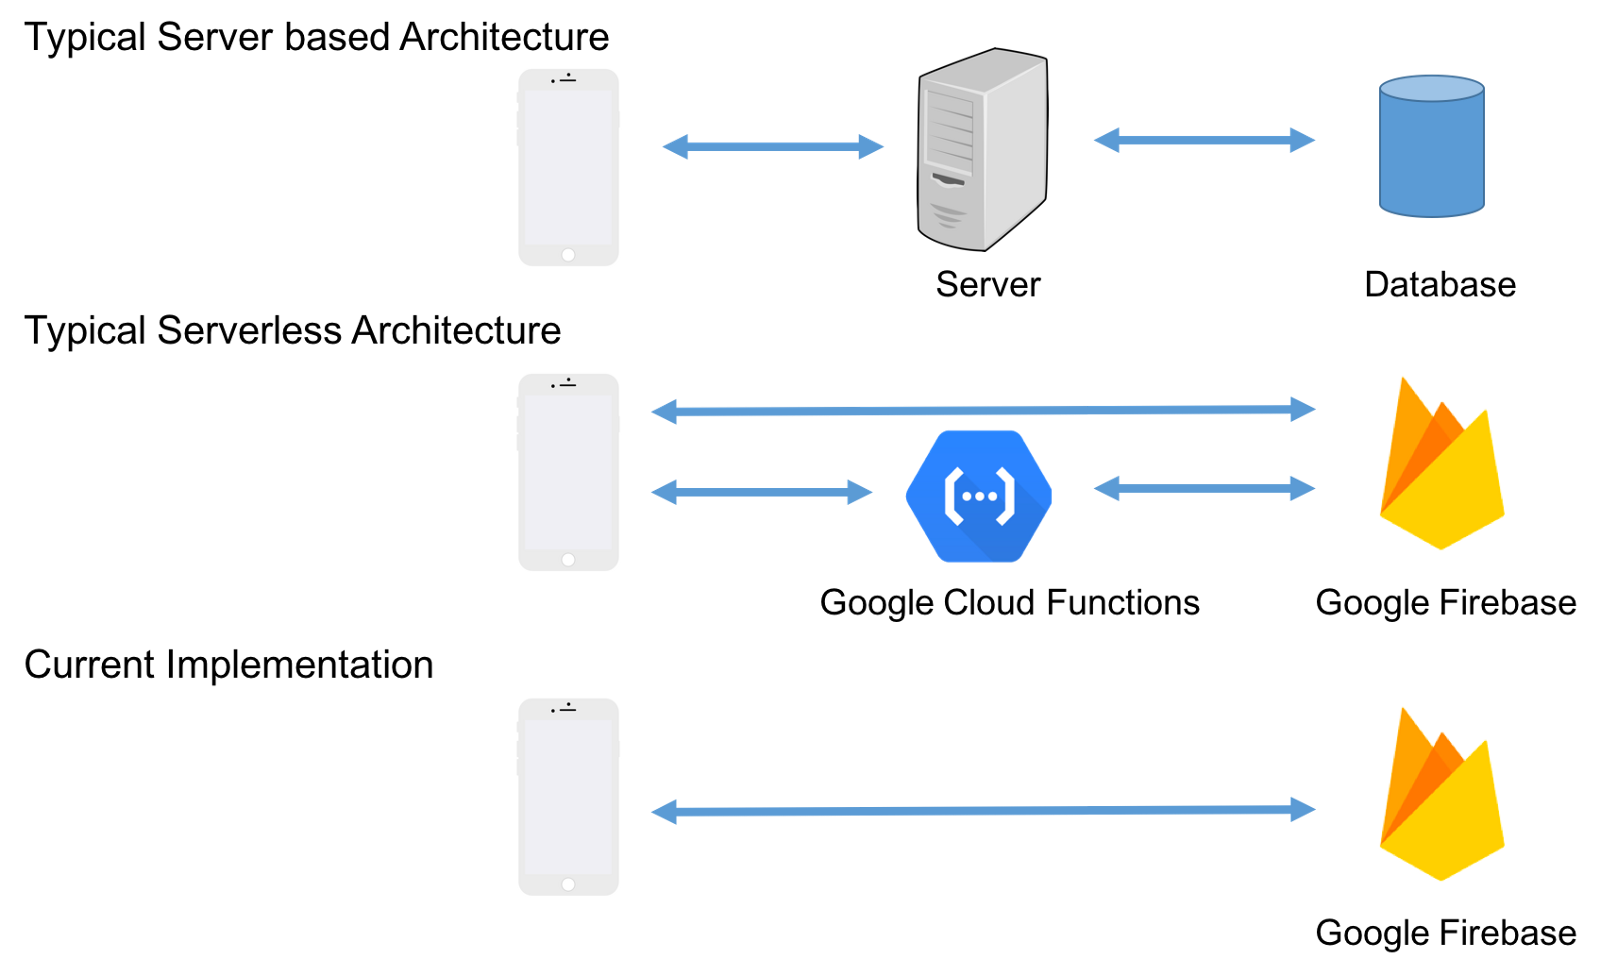
\includegraphics[width=0.9\textwidth]{images/architecture.png}
\end{figure}


\subsection{Web Application}
The web-application was designed with the intentionally of being easy to understand and highly navigable. For this the first section of the web-application to be implemented was the header component. The header component consists of a numbers of features, the name of the web-application is bold and centered as would be typically expected of a web-application of this type. Along with this are two dynamic features the page name and page icon, which change depending on which page the user is accessing. After this the header component features five static icons, An icon to link to the products page, an icon to route to user page (colour of icon is dynamic, changing as user login status changes), an icon that links to the user cart (badge displaying count changes as items entered changed), an icon linking an about page to describe the intention of the application and an icon routing to admin panels. 

\begin{figure}[h!]
    	\caption{Header component as is found in the web-application}
	\centering
	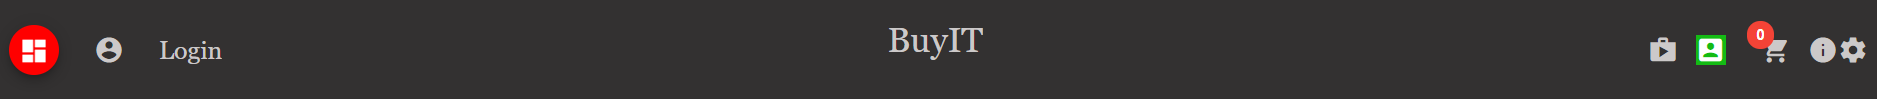
\includegraphics[width=0.9\textwidth]{images/header.png}
\end{figure}

\newpage
When first accessing the web-application users are routed to the "login" component. The "Login" component consists of an Angular Material form with two inputs, E-mail and Password to be used for logging in using traditional methods, a button for logins using a Google account and a link to redirect users who have yet to register to the "signup" component. The "signup component" consists of an Angular Material form featuring inputs for an e-mail and password. Both of these components feature a login button that is disabled until the input values in the form are considered to be valid, the restrictions on what constitutes a valid input are outlined when an error in input is made.

\begin{figure}[h!]
    	\caption{Login component as is found in the web-application}
	\centering
	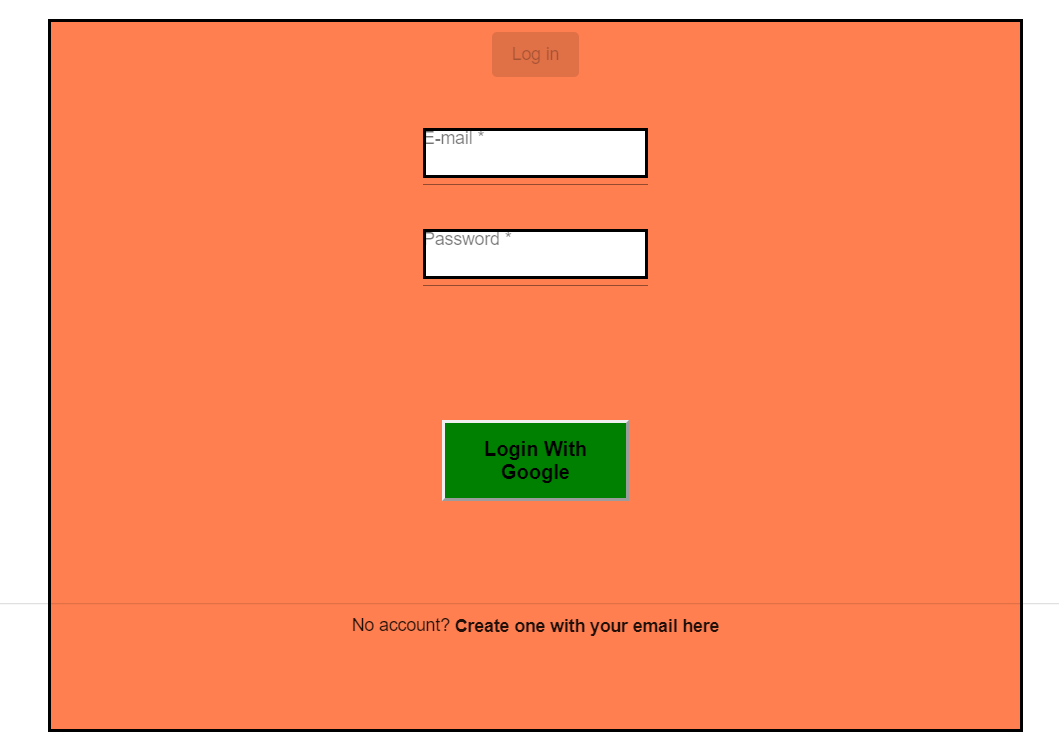
\includegraphics[width=0.9\textwidth]{images/login.png}
\end{figure}

\begin{figure}[h!]
    	\caption{Signup component as is found in the web-application}
	\centering
	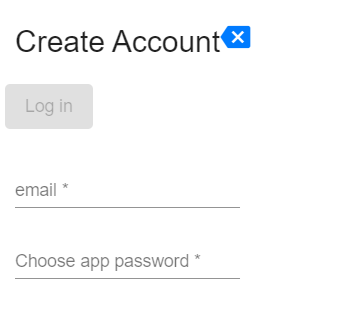
\includegraphics[width=0.9\textwidth, height=7cm]{images/signup.png}
\end{figure}

\\
After completing the login or registering as a new user, a standard user has access to four different components. The about page, the product listings page, the user information page and the user cart page. If an non-logged in user tries to access any of these pages then they are automatically re-routed to the login component. This was doing using a standard auth-guard-service. 

\begin{figure}[h!]
    	\caption{Auth-Guard-Service used to stop non logged in users accessing specified pages}
	\centering
	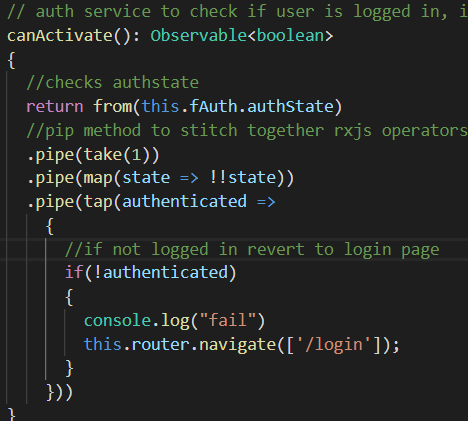
\includegraphics[width=0.9\textwidth, height=7cm]{images/authguard.png}
\end{figure}

\newpage
The about component is a simple HTML page, it features no back end functionality and is in place only to inform those that are not aware of the purpose of the web-application or for those interested in seeing which technologies were used in the creation of the web-application. The page consists of a small paragraph about the application and its developer and a series of links to the technologies used and the the github repository of the project. 

\\ \\
The user information page contains an angular material form that has four input fields (First name, surname, address and age). The first three inputs are given string values and the age field is given a number value. When these fields are correctly filled, the submit button which was initially disabled becomes ready for use. When the submit button is followed the information in the fields of the form, along with the email of the current user and the unique id assigned to the user is sent to the Firebase database as part of a collection of users. Also present on the user information page is a logout button that allows for the current user to be logged out if it is selected, the user is then routed back to the login page.



\begin{figure}[h!]
    	\caption{The User Information page as it appears in the web-application}
	\centering
	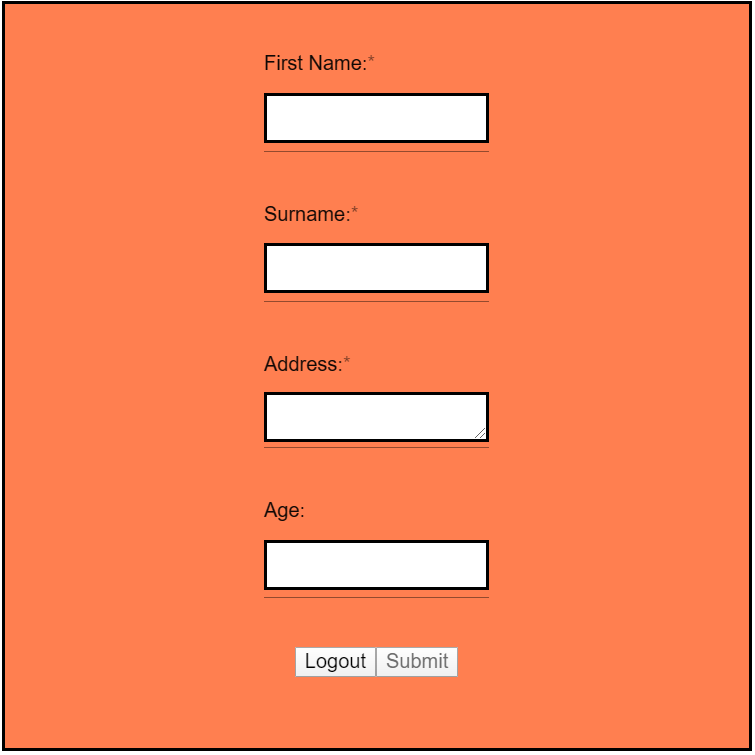
\includegraphics[width=0.9\textwidth, height=7cm]{images/uinfo.png}
\end{figure}
\begin{figure}[h!]
    	\caption{User collection and user document in Firebase database}
	\centering
	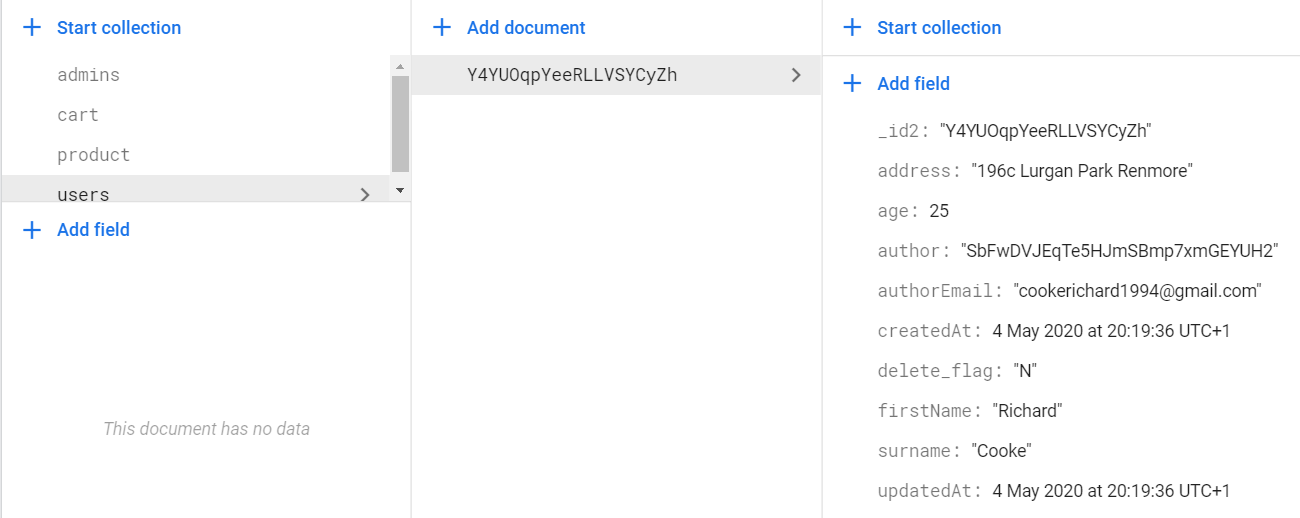
\includegraphics[width=0.9\textwidth, height=7cm]{images/usercol.png}
\end{figure}

\paragraph{}
The product listing page is made using two ng-templates. When the user first enters this page they are presented with a search bar on the top left corner(The functionality of the search bar however does not work correctly) and a listing of all the products stored within the Firebase database. Each row of the table constitutes a different product of the database. This was done by using a for loop to asynchronously loop through the data base create a row for for each document. The tables features four columns, the name of the product, the category of the product, the price of the product and a "view" button that changes to the alternative ng template of the page.
\newpage
\begin{figure}[h!]
    	\caption{The table of products as it appears to the user}
	\centering
	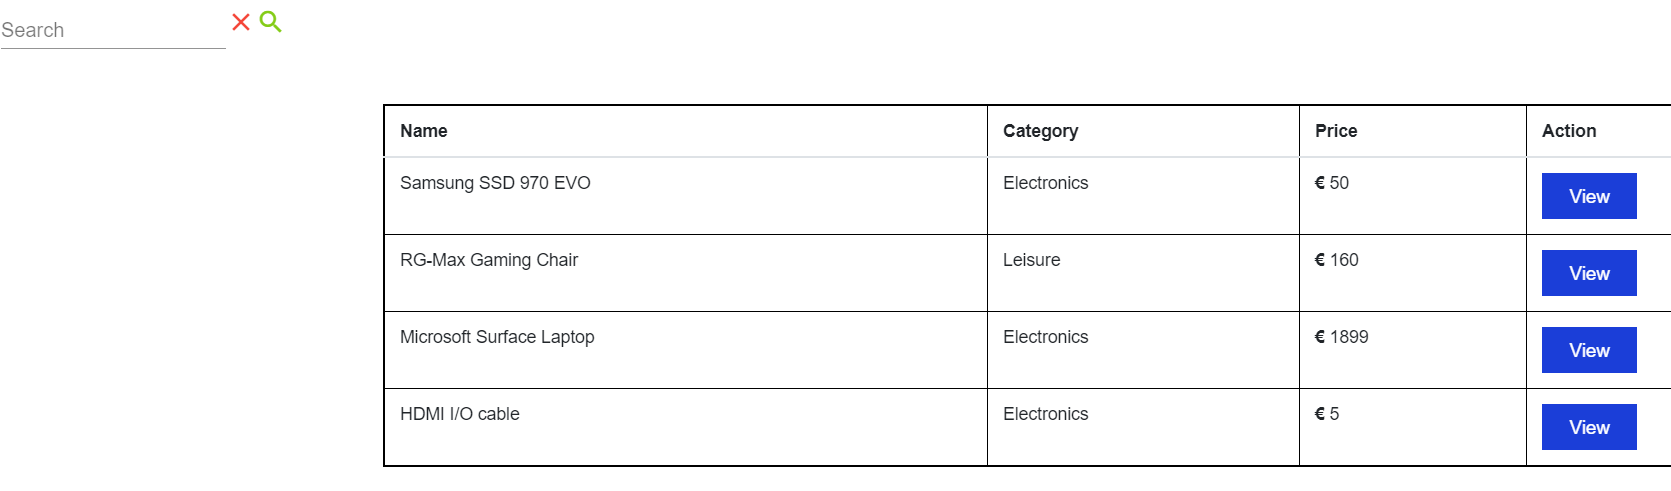
\includegraphics[width=12cm, height=7cm]{images/producttable2.png}
\end{figure}
\begin{figure}[h!]
    	\caption{How the table of products is constructed}
	\centering
	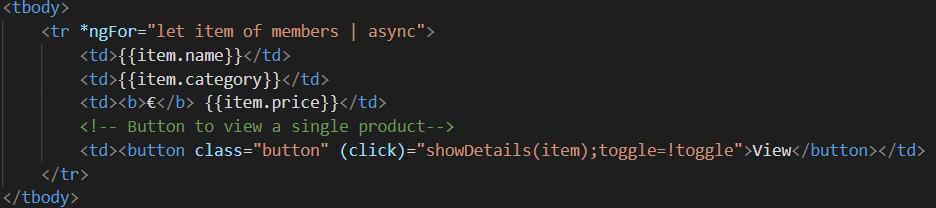
\includegraphics[width=12cm, height=7cm]{images/producttable.png}
\end{figure}

\newpage

\paragraph{}
The alternative ng-template which is called by the user selecting the aforementioned view button displays a single item display for the product that the user has selected the view button for. On this template the user is presented with all of the fields available in the previous templates table along with new information such as a long form description of the product an image of the product. Along with this is an "Add to Cart" button that uses back end functionality to pass the data of the product in view to the user cart and iterates the badge counter on the cart icon present on the web-applications header. Along with this is a review system in place for each product. Reviews are based on a "5 star" format where each user can rat the product from 0.5 to 5.0 stars. After the user has rated the product a review becomes present on screen featuring the unique ID of the user that posted the review and the rating to which they applied to the product. Above this the average of all the user reviews is displayed. If no review has been completed for a product then users will be met with a message informing them of such. 


\begin{figure}[h!]
    	\caption{Product with image displayed in product view}
	\centering
	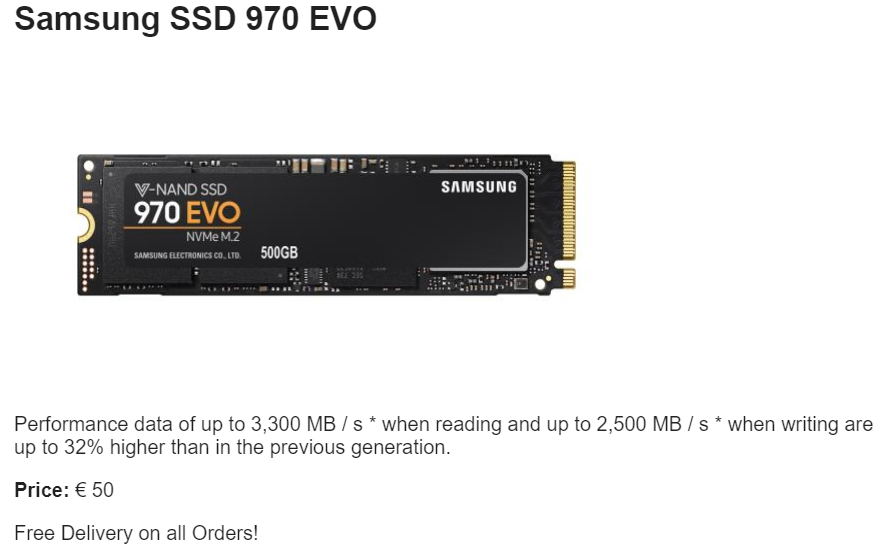
\includegraphics[width=0.9\textwidth, height=7cm]{images/productview.png}
\end{figure}
\newpage
\begin{figure}[h!]
    	\caption{Review section of the product view}
	\centering
	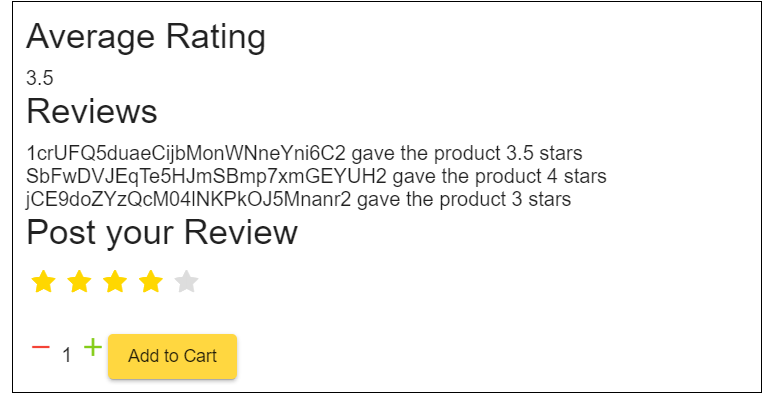
\includegraphics[width=0.9\textwidth, height=7cm]{images/review.png}
\end{figure}

\newpage
The cart page provides a similar view as the products page. All products within the cart are organized using a table. All the fields that were present in the products table are also present in the cart table along with the addition of a "Remove" button. The remove button allows for the selected product to be removed from the users cart. When an item is removed from the cart, the badge counter on the cart icon of the header is decremented by one. While all products when added to the cart are added to the same collection in the database, the user cart only displays items added by the current user, identified by the Firebase provided unique ID. At the bottom of the cart is the total price of all the items in the cart, along with this is a place order button which is not functional. 


\begin{figure}[h!]
    	\caption{How the cart is seen by the user}
	\centering
	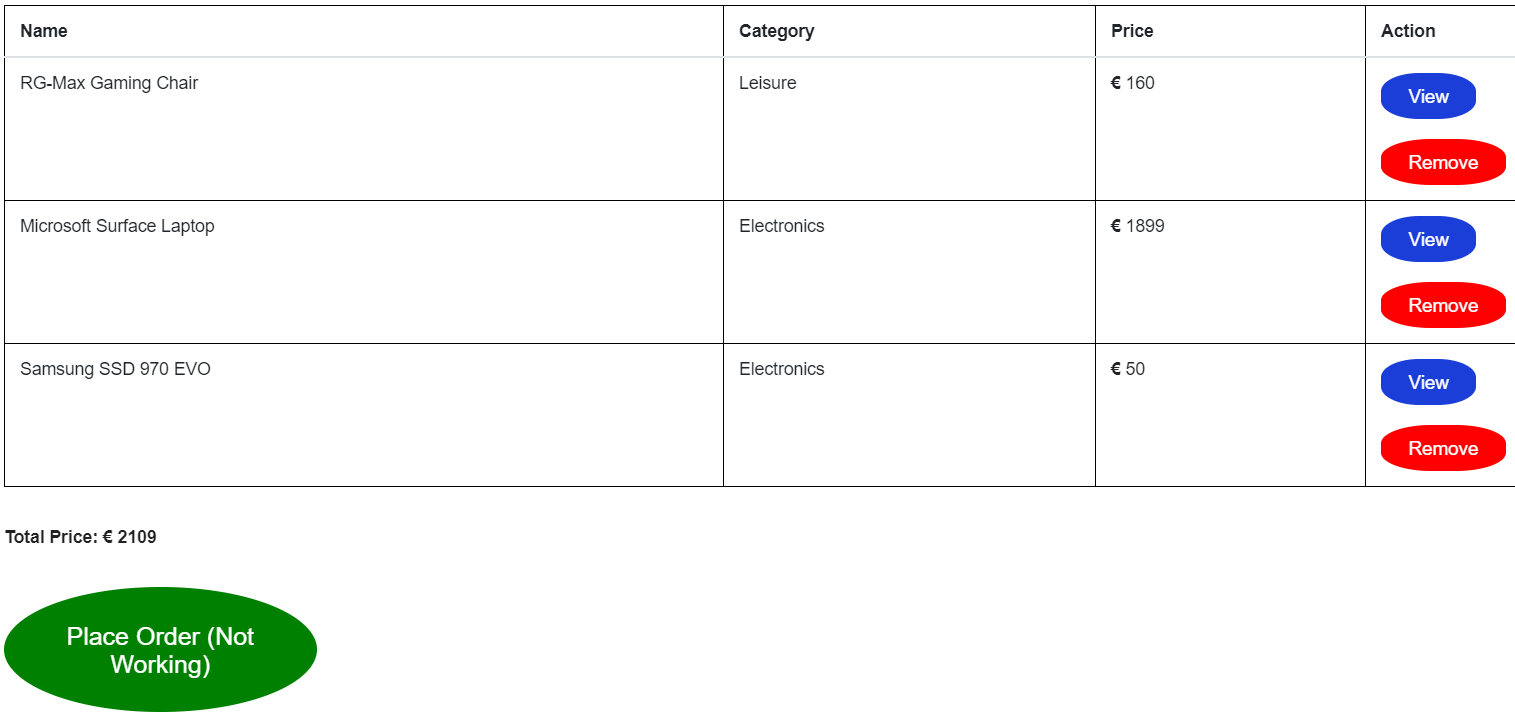
\includegraphics[width=12cm, height=7cm]{images/cartview.png}
\end{figure}
\begin{figure}[h!]
    	\caption{How the items of the cart are called where the current user added them}
	\centering
	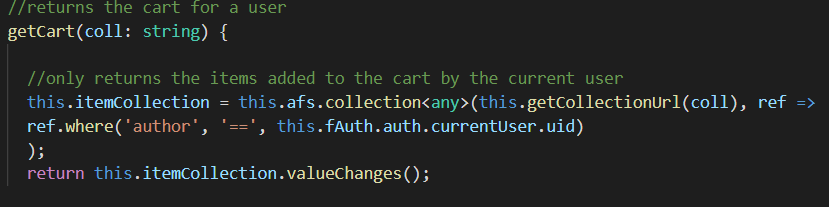
\includegraphics[width=12cm, height=5cm]{images/cartcode.png}
\end{figure}

\newpage
The cart page also shares the view option that is present in the products page. This view however is more limited than the view of the products page for an individual item. There is no option to review the item or add it to cart and instead this view is more for the user to ascertain the correct product is in the cart.

\\ \\
The final component available on the web-application is the admin panel. The admin panel is the subject of heavily restricted access, only users who have been granted access to the admins collection on the Firebase database can view this page. The assignment of admin status is done manually by those with access to the database. This restriction of access is accomplished by implementing a similar service to the auth-guard-service to restrict non-logged in users accessing pages. This time an admin-auth-guard-service is used, which provides tighter security. 
\begin{figure}[h!]
    	\caption{Admin Guard Service to prevent non Admins accessing Admin panel}
	\centering
	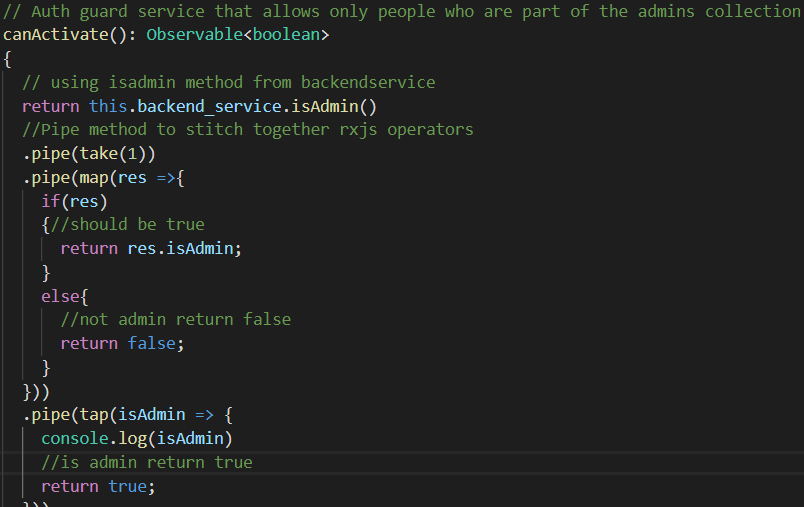
\includegraphics[width=12cm, height=5cm]{images/adminguard.png}
\end{figure}
\newpage
The Admin page consists of two tabs, the users tab and the products tab. The users tab returns a full list of users who have entered personal information using the user information page. This data is displayed in table format and features columns relating the the users unique ID, the users First Name, the users Surname and the users E-mail. The Admin has no control over this user data other than viewing privileges. The admin is able to sort the users list by the unique ID and is also able to change the amount of users on display using the paginator.


\begin{figure}[h!]
    	\caption{Admin view of users list}
	\centering
	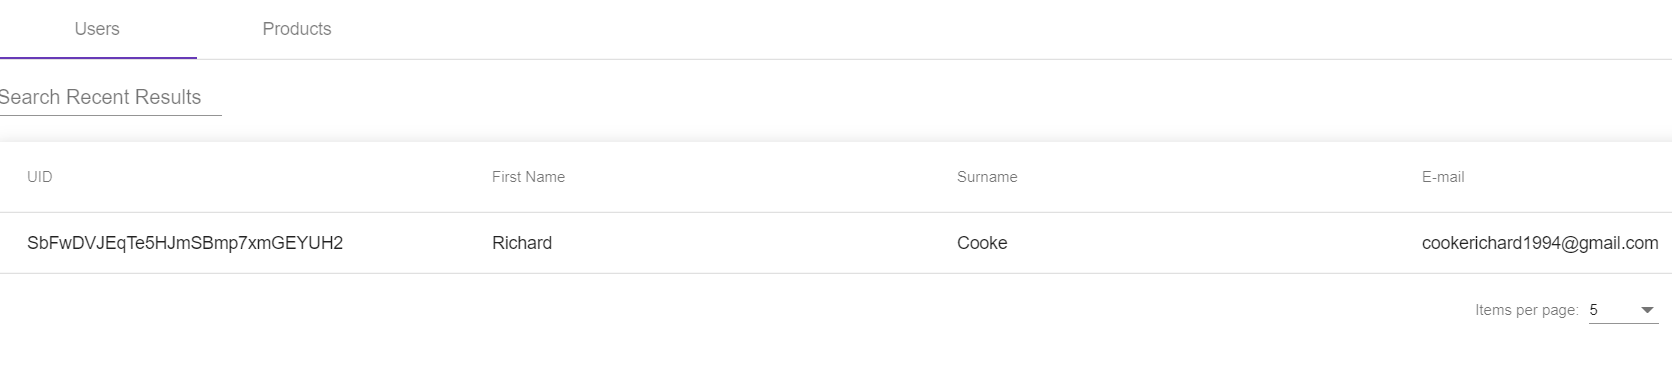
\includegraphics[width=15cm, height=7cm]{images/adminusers.png}
\end{figure}

The second tab, the products tab allows for most of the administrator functionality. Here the Admin can views a list of all products in the database in table format, can add new products, can edit products, can delete products, filter through the products and add or remove a picture to the product. There are four templates to the admin products view. Initially the view is set to the search mode were the admin can search through the products with a number of methods, included by narrowing the date using a ate picker although this is not fully functional. 
\newpage
\begin{figure}[h!]
    	\caption{Admin view of searching products}
	\centering
	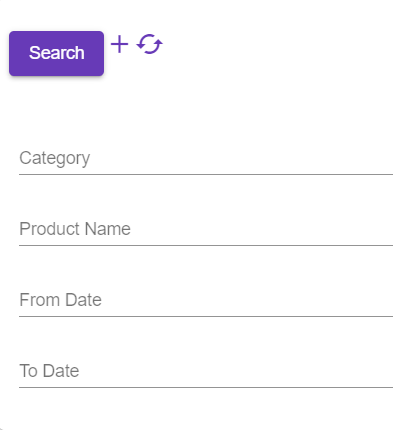
\includegraphics[width=10cm, height=6cm]{images/adminsearch.png}
\end{figure}

The next view is the list of products which is a table format and uses icons located at the end of the product for altering or removing the product in question. 

\begin{figure}[h!]
    	\caption{Admin view of products list}
	\centering
	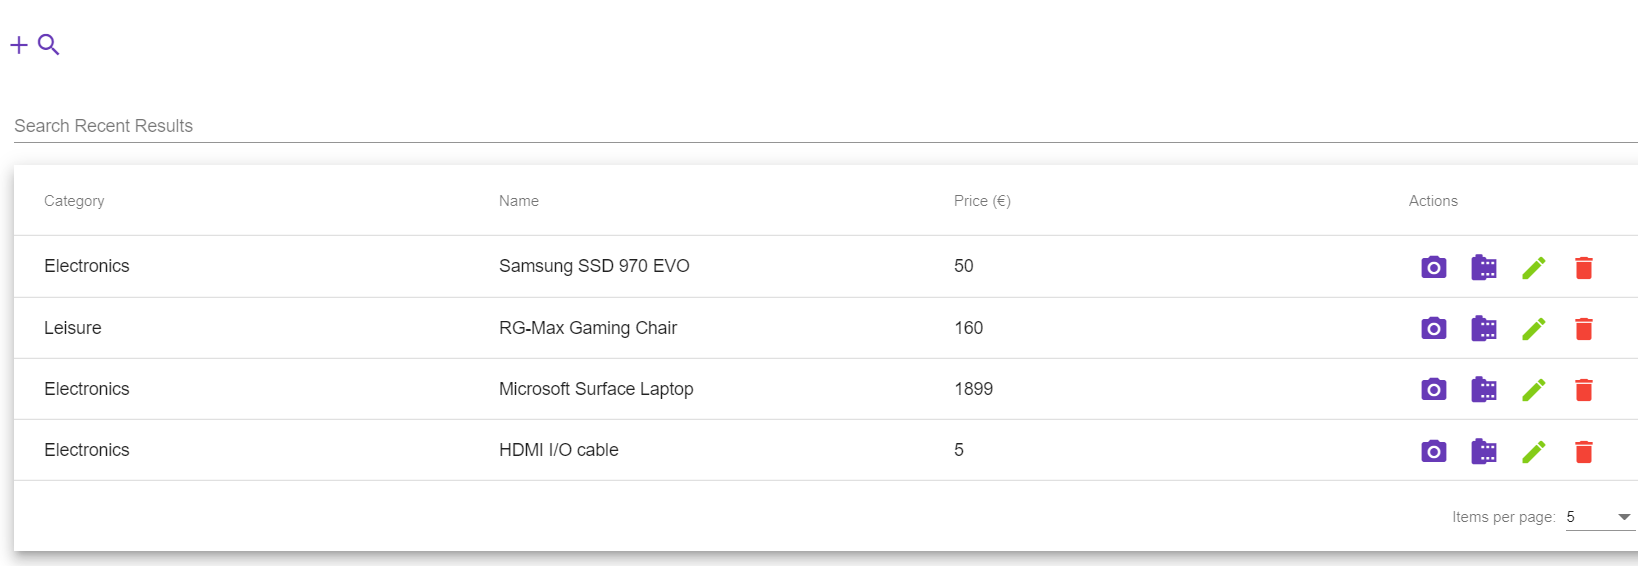
\includegraphics[width=15cm, height=7cm]{images/adminproducts.png}
\end{figure}

The Edit mode is accessed by selecting the pencil icon at the end of each product in the list view, it provides 4 fields of entry from an Angular material form where the previous data is carried across, an add button is used to update the information and a clear removes all information present in the data fields. The add mode uses the same view as the edit mode, except that the fields are initialized as empty and the add button creates a new product instead of updating an existing one.

\begin{figure}[h!]
    	\caption{Admin view of adding or editing a product}
	\centering
	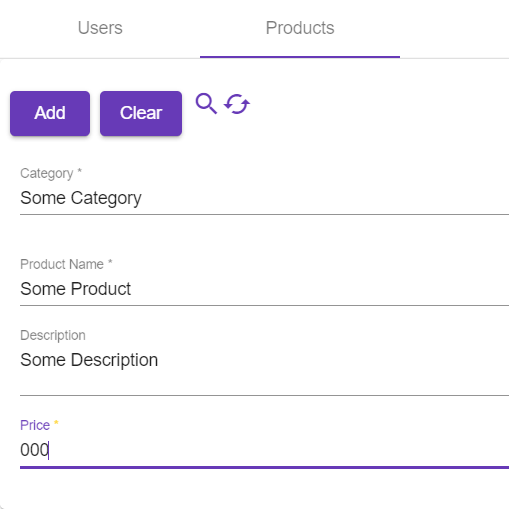
\includegraphics[width=10cm, height=6cm]{images/adminadd.png}
\end{figure}

\subsection{Functionality}
In this section we will look at the services within the application that act as a back end to the web-application. As previously mentioned, each component in Angular has a HTML file which provides the view and a typescript file which carries the pages functionality. I the case of this project most of the actual functionality is present in a service called backendservice.ts. This file is what links the angular application to the Firebase Database using the environment of the project. Backendservice.ts is made up mostly of reusable functions that are called by the typescript files of the Angular components. This done by importing the backendservice as part of the constructor for these typescript files.
\\
Most queries of the database are made by using a hard coded string that dives into a certain level of the Firebase database before entering the a collection that has been specified through a method that has been passed to it. The name of the collection that is to be queried is passed by the typescript file of the angular component on to the back end service which then appends it to the constant string and then sends a request to the database using this newly formed string.

\begin{figure}[h!]
    	\caption{getCollectionUrl method is used in every method that queries the Firebase database}
	\centering
	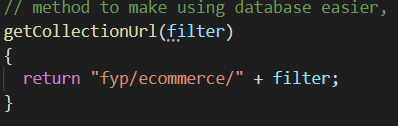
\includegraphics[width=10cm, height=6cm]{images/collurl.png}
\end{figure}
\newpage

\begin{figure}[h!]
    	\caption{For example the updateData method of setProducts.ts makes use of the backendservice method updateProducts}
	\centering
	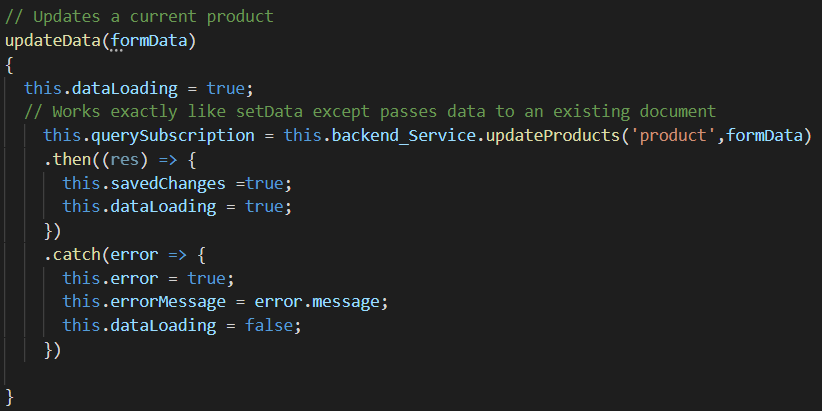
\includegraphics[width=10cm, height=6cm]{images/update.png}
\end{figure}
\begin{figure}[h!]
	\centering
	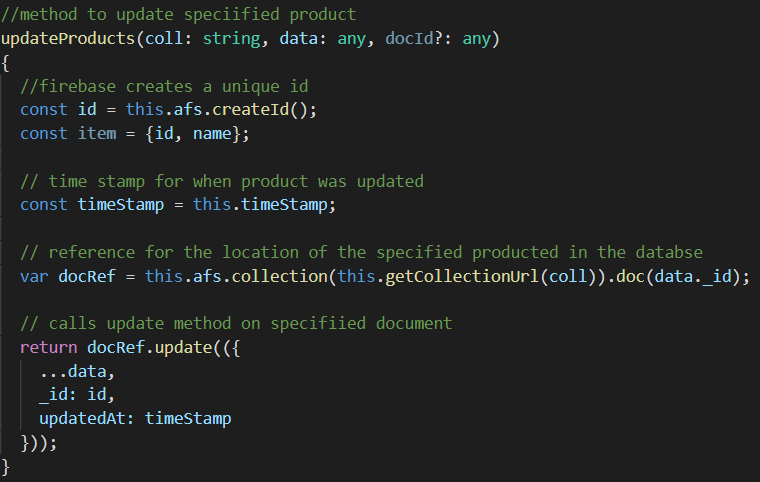
\includegraphics[width=10cm, height=6cm]{images/backendupdate.png}
\end{figure}

\newpage

\subsubsection{Review Functionality}
The functionality of using the review system is similar to creating a relationship like in an SQL databases with a many to many relationship. Unlike the other collections, it was determined to make the star collection a root collection which could dip into both the user collection and the product collection. This was done to establish the relationship of the collections. The review functionality is done by using an angular component as an inner-page and passing it two variables, the ID of the product being reviewed and the user ID of the reviewer, both of which are present when on the single product view. 
\begin{figure}[h!]
    	\caption{How the inner review page is called into product.html}
	\centering
	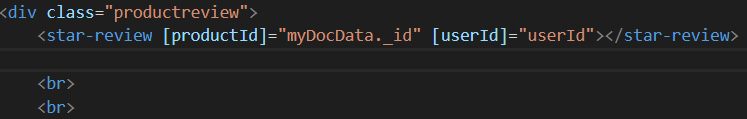
\includegraphics[width=15cm, height=6cm]{images/reviewcall.png}
\end{figure}


\subsubsection{Upload Image Functionality}
Like the Star Review page, the upload page is called as an inner page, this time as part of the set products page to be handled by the administrator. The upload page takes two parameters, the path of the file or image being uploaded and the id of the document this path is to be added to. Most of the functionality considered with file upload is adapted from the angular 2 handbook, which is referenced within the filesize.pipe.ts file which is used to handle the mathematics involved in file upload. The image upload occurs within the set product as one of the actions the administrator can take when creating or editing a product. When a product does not have an attached image the photo-reel icon is blacked out. After an image has been attached the blacked out image-reel is replaced with two icons a camera icon for viewing the uploaded image and a differently coloured photo-reel icon that when followed, removes the attached image of the specified document.

\begin{figure}[h!]
    \caption{Top: After an image is uploaded,
    Bottom: Before an image is uploaded.}
	\centering
	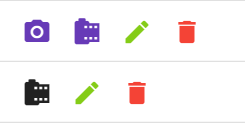
\includegraphics[width=10cm, height=4cm]{images/photoupload.png}
\end{figure}

\begin{figure}[h!]
    \caption{The startUpload method used to add an image file to a product}
	\centering
	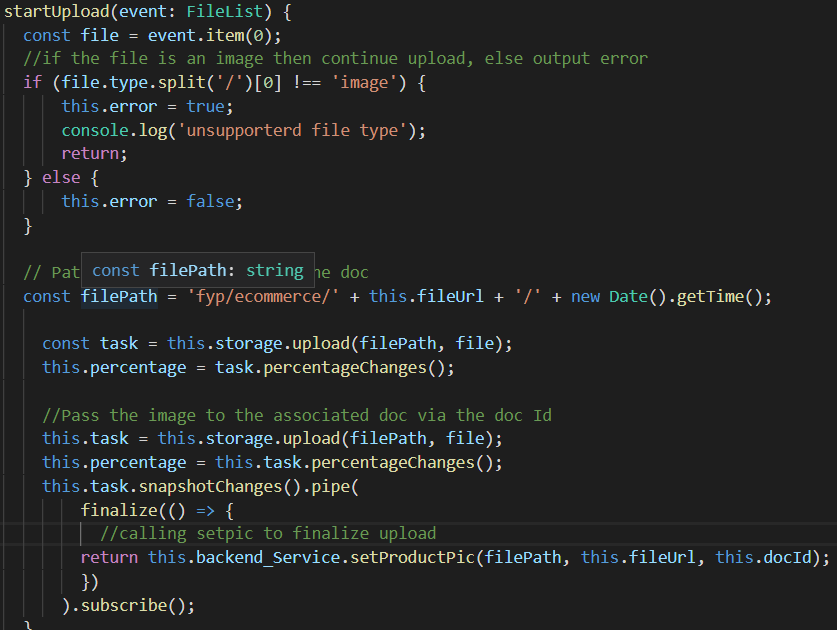
\includegraphics[width=15cm, height=15cm]{images/uploadmethod.png}
\end{figure}




















